\section{Asynchronmotor}
\renewcommand{\arraystretch}{0.9}  
\begin{minipage}{0.4\linewidth}
    \textbf{Eigenschaften:}
    \begin{itemize}
        \item meist verwendeter Elektromotor
        \item Drehfeld wird durch den Ständer erzeugt
        \item Drehmoment entsteht durch den im Läufer induzierten Strom
    \end{itemize}
\end{minipage} 
\begin{minipage}{0.5\linewidth}
    \textbf{Kennlinie Asynchronmotor}\newline
    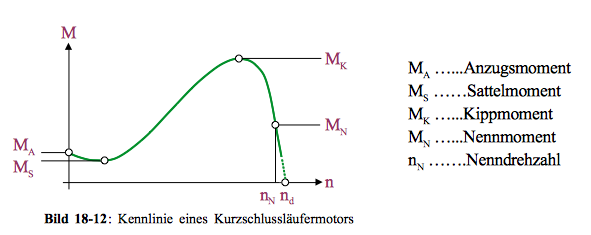
\includegraphics[scale = 0.6]{images/KennlinieASM}
\end{minipage}
\begin{multicols}{2}     
    \begin{minipage}{\linewidth}
        \textcolor{green}{Vorteil}:
        \begin{itemize}
            \item sehr einfacher Aufbau
            \item sehr robust und widerstandsfähig 
        \end{itemize}
    \end{minipage}
    
    \begin{minipage}{\linewidth}
        \textcolor{red}{Nachteil}:
        \begin{itemize}
            \item Extrem hoher Anlaufstrom \newline
            $\Rightarrow$ dies wird vermindert mit der Stern-Dreieck-Umschalt-Methode \newline
            (3 Mal mehr Leistung im Dreieckbetrieb)
        \end{itemize}
    \end{minipage}
\end{multicols}

\subsection{Aufbau Ständer}
    \begin{minipage}[b]{0.45\linewidth}
    	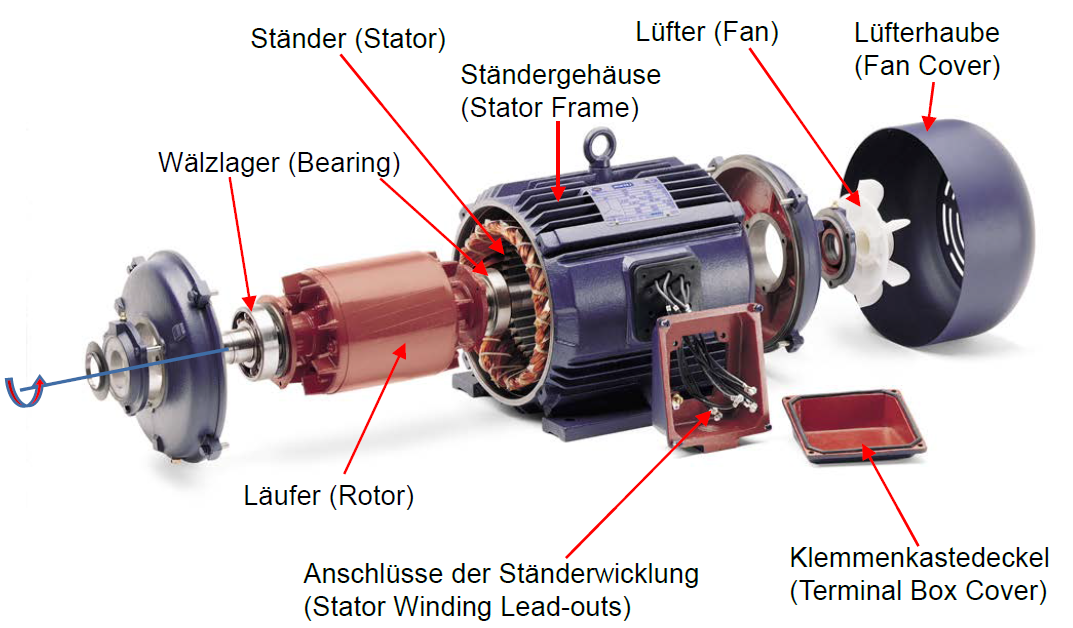
\includegraphics[scale = 0.3]{images/AsynchronmotorAufbau}
    \end{minipage}
    \begin{minipage}[b]{0.28\linewidth}
    	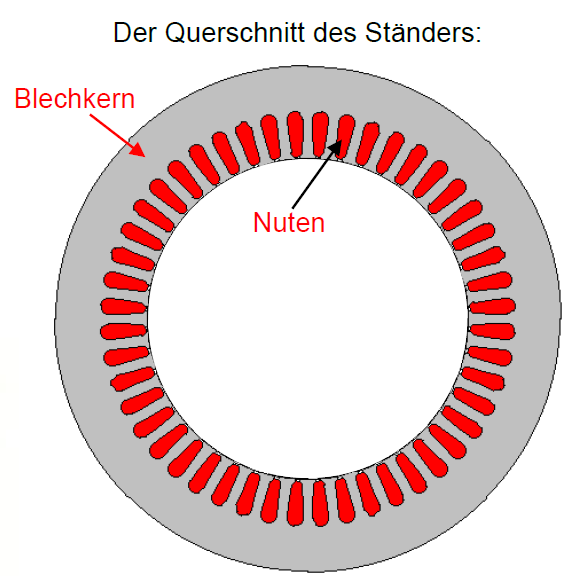
\includegraphics[scale = 0.3]{images/AQuerschnitt}
    \end{minipage}
    \begin{minipage}[b]{0.33\linewidth}
    	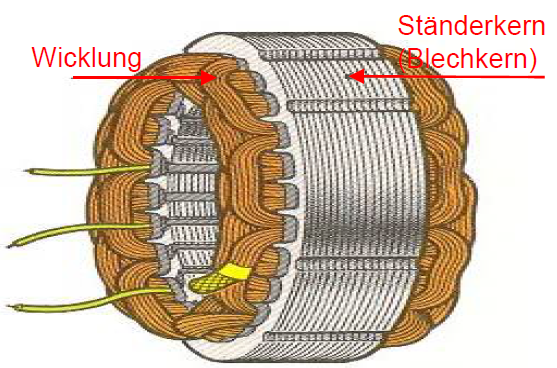
\includegraphics[scale = 0.4]{images/AsynchronmotorStaenderkern}
    \end{minipage}\\
    \subsection{Aufbau Läufer}
    \begin{multicols}{3}
        \begin{minipage}{\linewidth}
        	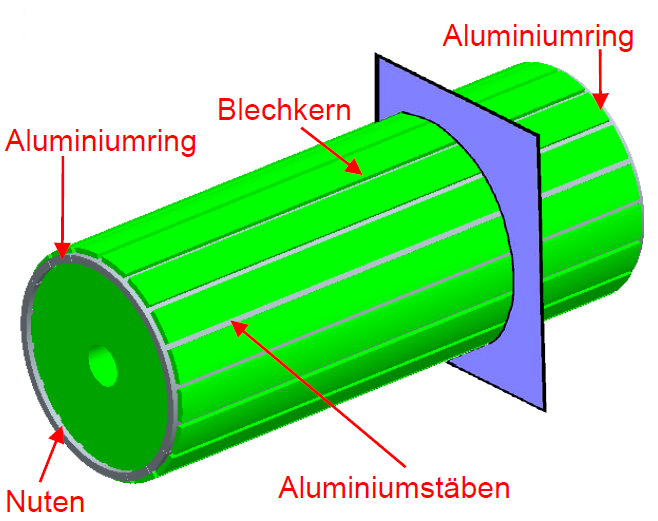
\includegraphics[width=\linewidth]{images/AsynchronRotor}
        \end{minipage}   
             
        \begin{minipage}{\linewidth}
        	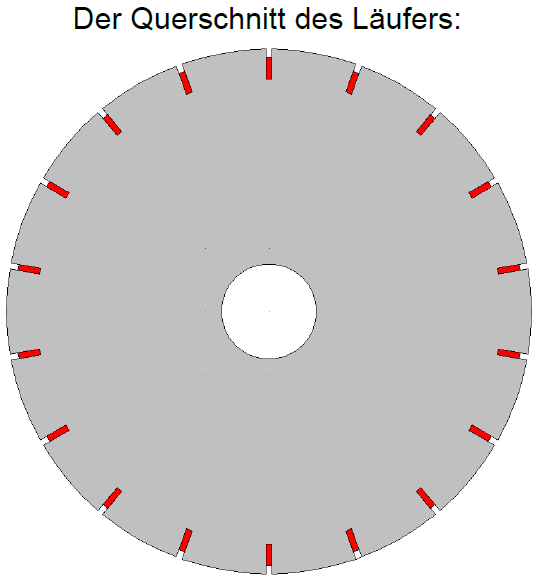
\includegraphics[width=0.7\linewidth]{images/QuerschnittAsynchronrotor}
        \end{minipage}  
              
        \begin{minipage}{\linewidth}
            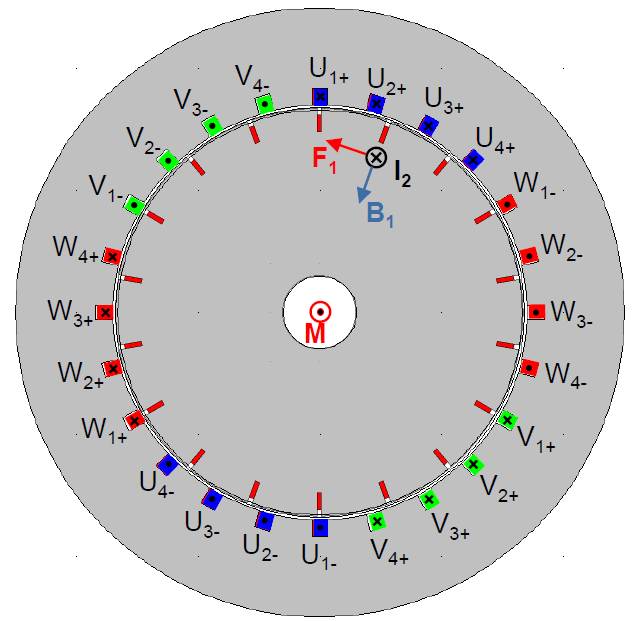
\includegraphics[width=\linewidth]{images/QuerschnittAmotor}
        \end{minipage}
    \end{multicols}
    Wirbelströme im Eisen entstehen durch die Induktion des Rotors in den Stator \newline
    $\Rightarrow$ Stator erwärmt sich.\newline
    Durch den Rillenaufbau des Stators können diese Wirbelströme bzw. die Temperaturansteigung minimiert werden.
    \\
    Schlupf $\widehat{=}$ Abweichung zu der Synchronen Drehzahl 
    \clearpage
    \pagebreak

\subsection{Formeln Läufer}
\renewcommand{\arraystretch}{1}
\subsection{Modell der Asynchronmaschine}\vspace{-1cm}
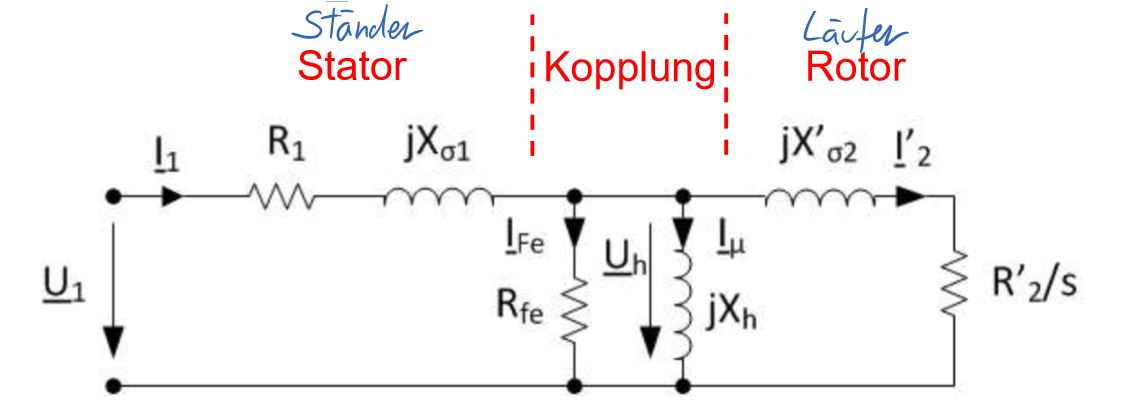
\includegraphics[scale = 0.6]{images/ModelASM}
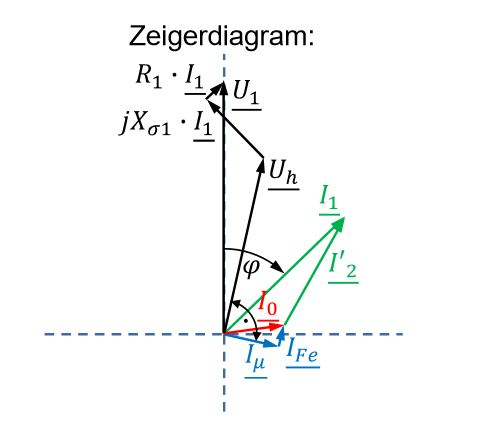
\includegraphics[scale = 0.8]{images/ModelASMZeiger}

\begin{longtable}{| p{.50\textwidth} | p{.45\textwidth}|}
    \hline
    \textbf{Grundgleichungen:}\newline
    \[ \underline{I_1}= \underline{I_{Fe}}+\underline{I_\mu}+\underline{I'_2} \approx \underline{I'_2} \]
    \[ \underline{U_1}= R_1 \cdot \underline{I_1}+jX_{\sigma 1}\cdot \underline{I_1}+ \underline{U_h} \approx \underline{U_h} \]
    \textbf{Übersetzungsverhältnis:}\newline
    \[ u=\frac{N_1 \cdot k_{w1}}{N_2 \cdot k_{w2}}\]
    \[ \underline{I'_2}=\underline{I_2} \cdot u \]
    \[ R'_2 = R_2 \cdot u^2 \]\vspace{-0.3cm}&
    N = Windungszahl \newline
    $ k_w $ = Wicklungsfaktor \newline
    $ R_1, X_{\sigma 1} $= Widerstand und Streureaktanz des Stators \newline
    $ R_2, X_{\sigma 2} $= Widerstand und Streureaktanz des Rotors \newline
    $ R_{Fe} $= Eisen-Verlustwiderstand \newline
    $ X_h $= Hauptreaktanz \newline
    $ U_h $= innere Spannung \newline
    $ I_\mu $= Magnetisierungsstrom
    \\ \hline      
\end{longtable}

    \begin{longtable}{| p{.30\textwidth} | p{.35\textwidth} | p{.25\textwidth} |}
    	\hline
    	\textbf{Induzierte Spannung} &
        \[ U_i = 4.44\cdot f\cdot w\cdot\xi\cdot\phi \] &
        f $\widehat{=}$ Frequenz \newline
        w $\widehat{=}$ Windungszahl \newline
        $\xi$ = Wicklungsfaktor \newline
        $\phi$ = Magnetischer Fluss
        \\ \hline
        
        \textbf{Elektromagnetische Kraft}	&
        \begin{equation*} \vec{F_2} = l_2\cdot\vec{I_2}\times\vec{B_1}\end{equation*} &
        $ B_1 $= Flussdichte\newline
        $ I_2 $= Strom Rotor        
        $ l_2 $= länge Rotor\newline
        \\ \hline
        
        \textbf{Mech. Drehmoment}	&
        \begin{equation*}\vec{M_2} = \vec{r_2}\times\vec{F_2}\end{equation*}&
        $ r_2 $= radius Rotor
        \\ \hline
        
        \textbf{Drehzahl}&
        \[ n_1= \frac{f_1}{p}\]
        \[ n_2=n_1 - n \]&
        n = Drehzahl des Läufers \newline
        $n_1$ = Synchrondrehzahl \newline
        $ n_2 $ = Relativdrehzahl
        \\ \hline
        
        \textbf{Schlupf}&
        \[ s= \frac{n_2}{n_1}=\frac{n_1-n}{n_1}=\frac{f_2}{f_1} \]&
        $ f_1 $ = Frequenz Drehfeld \newline
        $ f_2 $ = Frequenz Anker \newline
        Synchroner Lauf: s = 0 \newline
        Stillstand: s = 1
        \\ \hline 
        
        \textbf{Induzierter Strom}&
	     \[I_1=\frac{U_{1}}{\sqrt{\left(\dfrac{R_2^\prime}{s}\right)^2+X_{2\sigma}^{\prime 2}}}\] 
         \[ I_2 = \frac{U_{i20}}{\sqrt{\left(\dfrac{R_2}{s}\right)^2+X_{2\sigma}^2}} \]&
         \[ R_2^\prime= X_{2\sigma}^{\prime}\cdot s_k \]
         \\ \hline
            
        \textbf{Verluste Drehmoment}\newline
        \tabbild[scale = 0.3]{images/PVerluste}&
        \[ P_{D1}=P_m+P_{C22} \]
        \[ P_{D1}=2\cdot\pi\cdot n_1\cdot M\]
        \[ P_N = P_m = 2\cdot\pi\cdot n\cdot M \]
        \[ M = \frac{1}{2 \pi n_1}\frac{P_{Cu2}}{s} \]&
         $ P_1 $ - primäre Netzleistung \newline
         $ P_{Cu} $ - Ohmsche Verluste \newline
         $ P_{Fe} $ - Blechkernverluste \newline
         $ P_{D1} $ - Drehfeldleistung \newline
         $ P_m $ - mechanische Leistung \newline
         $ P_N $ - Nennleistung \newline
         $ P_R $ - Reibungsverluste und Lüftung \newline
         $ P_m^{\,\prime} $ - mech. Nutzleistung \newline
         M - Drehmoment
        \\ \hline
        
        \textbf{Funktion Drehmoment} \newline
        \tabbild[scale = 0.4]{images/FunktionDrehmoment}&
        \[ M=\frac{1}{2\pi n_1}\frac{\textcolor{blue}{P_{Cu2}}}{s} \]
        \[= \frac{\textcolor{blue}{q_2}}{2\pi n_1}\cdot \textcolor{green}{I_2^2}\cdot\frac{\textcolor{blue}{R_2}}{s} \]
        \[= \frac{q_2}{2\pi n_1}\textcolor{green}{\frac{U_{i20}^2}{(R_2/s)^2+X_{2\sigma}^2}}\frac{R_2}{s} \]&
        \textcolor{blue}{M-Kennlinie} \newline
        \textcolor{yellow}{Motorbetrieb} \newline
        \textcolor{green}{Generator-Betrieb} \newline \newline
        $ q_2 $= Anz. Phasen der \newline Rotorwicklung\newline
        \\ \hline
        
        \textbf{Anlauf} \newline
        \tabbild[scale=0.4]{images/ASMAnlauf}&
        \[ M=\frac{q_1}{2\pi n_1}\cdot \frac{U_1^2}{(R_2'/s)^2+X_{2\sigma}^{'2}}\cdot\frac{R_2'}{s} \]
        \[ s_K=\frac{R_2'}{X_{2\sigma}'} \]
        \[ M_K= \frac{q_1}{4\pi n_1}\cdot\frac{U_1^2}{X'_{2\sigma}} \]&
        $ q_1 $= Anz. Phasen der \newline Statorwicklung\newline
        \\ \hline
        
        \textbf{Klosssche Gleichung}\newline
        Anlauf $\rightarrow$ s = 1&
        \[ \frac{M}{M_k}=\frac{2}{\frac{s}{s_k}+\frac{s_k}{s}} \]
        \[ \frac{1}{s} s_k^2 - \frac{2 M_k}{M}s_k+s=0 \]&
        $ s_k $= Kippschlupf\newline
        $ s_k > s $\newline
        $ M_k $= Kippmoment\newline
        $ M_k > M$
        \\ \hline        
              
    \end{longtable}
\clearpage
    \subsubsection{Leerlauf}
    \begin{multicols}{2}
        \begin{minipage}{\linewidth}
            Im Leerlauf wird die Asynchronmaschine an der \newline Welle nicht belastet.
            \[ R_1 << R_{Fe} \qquad X_{\sigma 1} << X_h\]
            \textbf{Ersatzschaltbild}\newline
            \tabbild[scale=0.9]{images/ASMLeerlauf}
        \end{minipage}
        
        \begin{minipage}{\linewidth}
            \tabbild[scale=1]{images/ASMLeerlaufZeiger}
        \end{minipage}
    \end{multicols} 
    \begin{longtable}{| p{.50\textwidth} | p{.45\textwidth}|}
        \hline
         \textbf{Synchronlauf \quad s=0} \newline
         \begin{minipage}{0.5\linewidth}    
         s = 0 \newline
         $ f_2 = 0 $\newline
         $ I_2 = I_{2max} = 0$\newline\newline
        \end{minipage}
         \tabbild[scale = 0.3]{images/FlussSynchron}&
         \textbf{Grundgleichungen}\newline
         $ \underline{I_0}=\underline{I_{Fe}} + \underline{I_\mu} $\newline
          $ cos(\varphi_0)= \dfrac{P_0}{U_0 \cdot I_0} $\newline
          $ R_{Fe}=\dfrac{U_0}{I_{Fe}}=\dfrac{U_0}{I_0 \cdot cos(\varphi_0)} $\newline
           $ X_h = \dfrac{U_0}{I_\mu}=\dfrac{U_0}{I_0 \cdot sin(\varphi_0)} $
         \\ \hline
    \end{longtable}
    
      \subsubsection{Kurzschluss}
          \begin{multicols}{2}
              \begin{minipage}{\linewidth}
                  Im Kurzschluss wird der Rotor der \newline Asynchronmaschine blockiert. (s=1)
                  \[ R_1 << R_{Fe} \qquad X_{\sigma 1} << X_h\]
                  \textbf{Ersatzschaltbild}\newline
                  \tabbild[scale=0.8]{images/ASMKurzschluss}
              \end{minipage}
              
              \begin{minipage}{\linewidth}
                  \tabbild[scale=1]{images/ASMKurzschlussZeiger}
              \end{minipage}
          \end{multicols}   
          
     \begin{longtable}{| p{.50\textwidth} | p{.45\textwidth}|}  
         \hline
         \textbf{Stillstand \quad s=1}\newline 
         \begin{minipage}{0.5\linewidth} 
             s = 1 \newline  
             $ f_2 = f_1 $  \newline 
             $I_2 = I_{2max} = \dfrac{U_{i20}}{\sqrt{R_2^2+X_{2\sigma}^2}}$\newline\newline
            \end{minipage}
        \tabbild[scale=0.3]{images/FlussStillstand}&
        \textbf{Grundgleichungen}\newline
         $ cos(\varphi_K)= \dfrac{P_K}{U_K \cdot I_K} $\newline
        $ R_1 + R'_2 = \dfrac{U_R}{I_K} = \dfrac{U_K \cdot cos(\varphi_K)}{I_K} $\newline
        $ X_{\sigma 1}+ X'_{\sigma 2}= \dfrac{U_X}{I_K}=\dfrac{U_K \cdot sin(\varphi_K)}{I_k} $
        \\ \hline
%         \textbf{4Q- Umrichter} \quad FU = Frequenzumrichter\newline
%         \tabbild[scale=0.8]{images/4QSchema}&
%          \newline
%         \tabbild[scale=0.8]{images/4QMn}
%         \\ \hline
    \end{longtable}
    \clearpage
